% Chương Quy trình ETL và kho dữ liệu
% Bảng trong latex/bang/etl_*.tex do python/tao_bang_tex_etl.py sinh từ nhật ký ETL (python/etl_nhat_ky.py).
% Hình etl_luong.png do python/ve_so_do_etl.py vẽ, hình luoc_do_sao.png do python/ve_luoc_do_sao.py vẽ từ DDL thật của kho.
% Nội dung thiết kế bám mục 3.2, 3.3 và kết quả bám mục 4.2 của báo cáo trên Google Doc.
\section{Quy trình ETL và kho dữ liệu}

Chương này mô tả cách nhóm lấy dữ liệu bán hàng của CompanyX, làm sạch rồi đưa vào kho dữ liệu \texttt{CompanyX\_DW} để phân tích. Quy trình này gọi là ETL: lấy dữ liệu ra (Extract), làm sạch và chuyển đổi (Transform), đưa vào kho (Load). Hình~\ref{fig:etlluong} tóm tắt toàn bộ luồng này.

\begin{figure}[H]
\centering
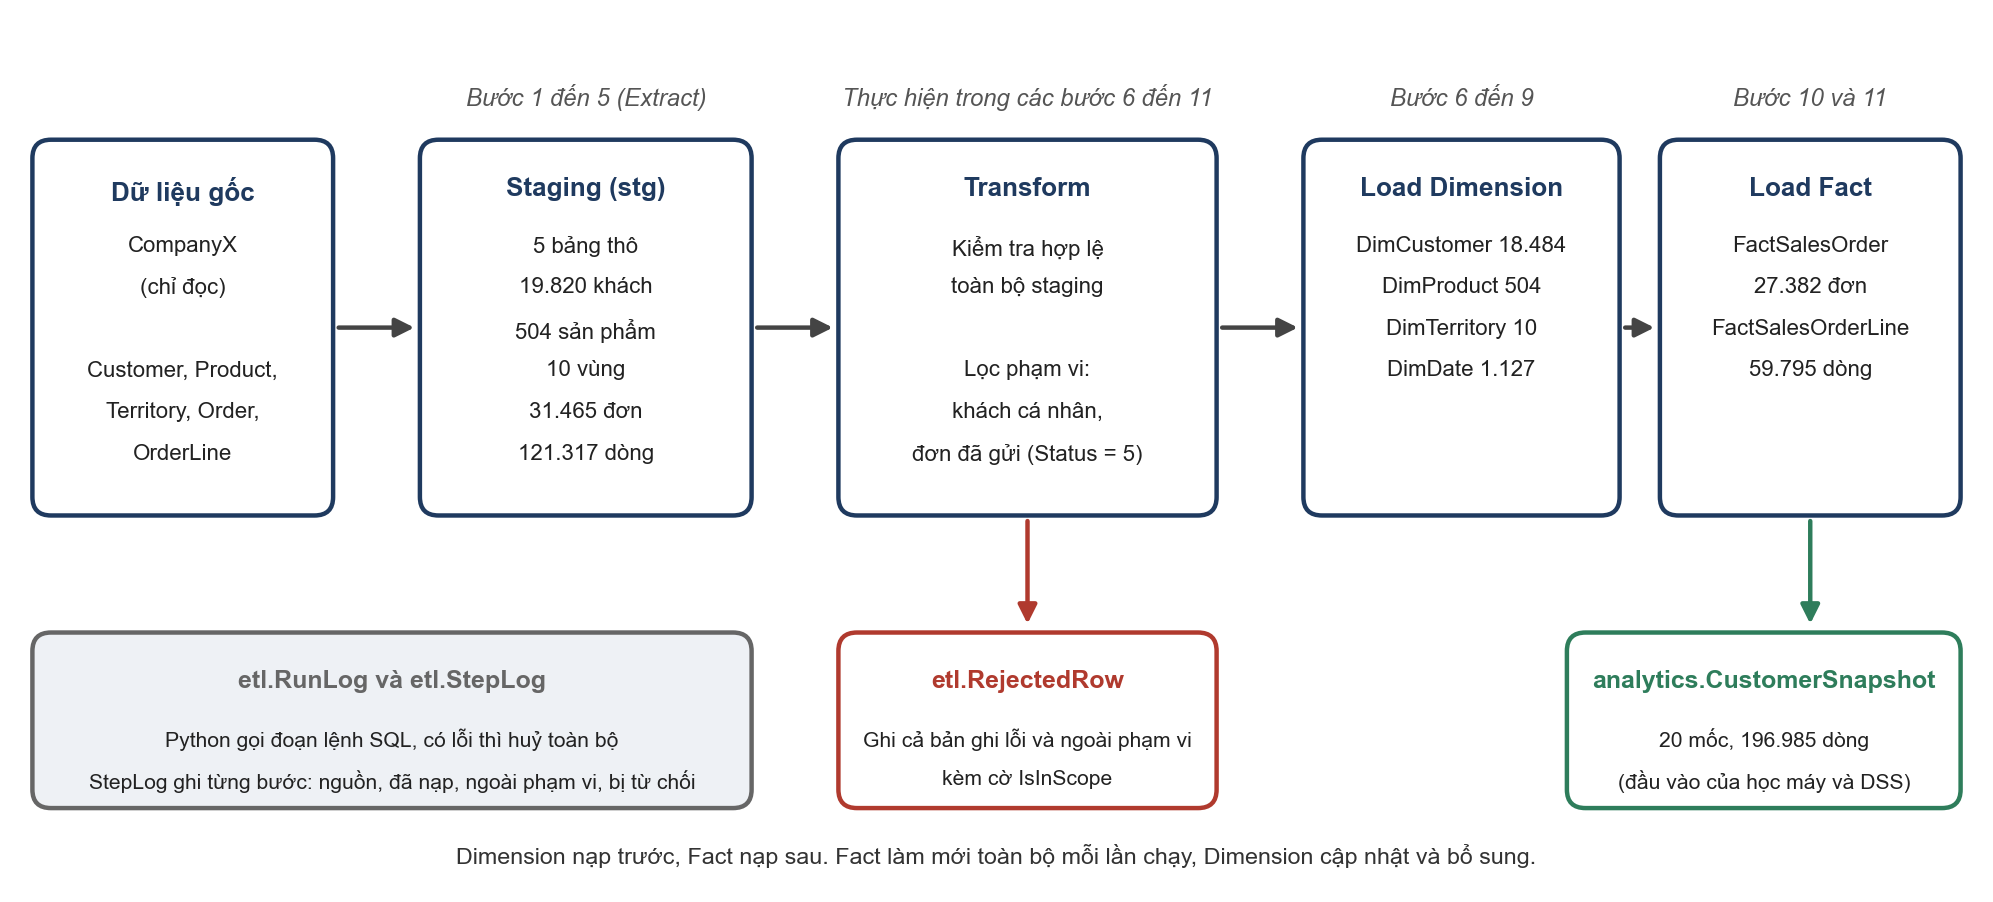
\includegraphics[width=0.8\textwidth]{etl_luong.png}
\caption{Luồng ETL từ dữ liệu gốc đến bảng Snapshot}
\label{fig:etlluong}
\end{figure}

\subsection{Khảo sát dữ liệu nguồn}
Trước khi thiết kế, nhóm xem kỹ cơ sở dữ liệu gốc bằng truy vấn SQL (Bảng~\ref{tab:khaosat}).

\begin{table}[H]
\centering
\caption{Kết quả xem dữ liệu gốc và quyết định của nhóm}
\label{tab:khaosat}
\footnotesize
\begin{tabular}{p{2.7cm}p{7.8cm}p{4.2cm}}
\toprule
Câu hỏi & Nhóm tìm thấy & Nhóm quyết định \\
\midrule
Dữ liệu là gì & CompanyX sản xuất xe đạp, đồng thời bán linh kiện, phụ kiện và trang phục. Cơ sở dữ liệu có 72 bảng về sản xuất, mua hàng và bán hàng. Các đơn được đặt từ 31/05/2011 đến 30/06/2014. Người mua gồm khách cá nhân (cột \texttt{PersonID} có giá trị) và cửa hàng đại lý (cột \texttt{StoreID} có giá trị) & Chỉ dùng phần bán hàng và khách cá nhân \\
Các bảng nối nhau ra sao & Mỗi đơn có một dòng tổng và nhiều dòng chi tiết (mỗi dòng là một sản phẩm), nối bằng \texttt{SalesOrderID}. Sản phẩm thuộc một nhóm nhỏ, nhóm nhỏ thuộc một nhóm lớn & Làm một bảng cho đơn, một bảng cho dòng chi tiết, và các bảng mô tả \\
Điểm cần lưu ý & \texttt{Status} bằng 5 nghĩa là đơn đã gửi. Ngày gửi luôn sau ngày đặt đúng 7 ngày. Tổng tiền đơn bằng tiền hàng cộng thuế và phí vận chuyển. Tháng 6/2014 có 930 đơn nhưng không có xe đạp nào. Có 6 đơn và 75 dòng chi tiết sai quy tắc & Chỉ lấy đơn đã gửi. Chỉ dùng ngày chốt $T$ khi dữ liệu đã có đến ngày $T+97$ (90 ngày theo dõi cộng 7 ngày gửi hàng). Loại các dòng sai quy tắc \\
\bottomrule
\end{tabular}
\end{table}

\subsection{Kiến trúc và luồng xử lý}
Quy trình chỉ đọc dữ liệu gốc, không sửa gì ở đó. Dữ liệu đi qua ba chặng như trong Hình~\ref{fig:etlluong}. Chặng một sao chép nguyên bản sang một vùng tạm gồm năm bảng (gọi là staging, tên \texttt{stg}). Chặng hai kiểm tra và lọc đúng phạm vi cần phân tích. Chặng ba đưa dữ liệu vào bốn bảng mô tả và hai bảng giao dịch của kho. Sau cùng, bảng \texttt{analytics.\allowbreak CustomerSnapshot} tóm tắt cách mua của từng khách để làm đầu vào cho học máy.

Python gọi một đoạn lệnh SQL lưu sẵn tên \texttt{etl.usp\_\allowbreak FullLoad} để làm hết các việc trên. Nếu có lỗi thì mọi thay đổi bị huỷ như chưa từng chạy (transaction). Cách làm này gần với ELT hơn ETL cổ điển: nạp dữ liệu thô vào vùng tạm trước, rồi biến đổi bằng SQL ngay trong SQL Server. Hai bảng \texttt{etl.RunLog} và \texttt{etl.StepLog} ghi lại các lần chạy, đóng vai trò siêu dữ liệu (metadata) của quá trình ETL.

\subsection{Thiết kế kho dữ liệu}
Kho được thiết kế theo mô hình hình sao. Ở giữa là bảng sự kiện (Fact), ghi các giao dịch cần đo. Xung quanh là các bảng chiều (Dimension), cho biết giao dịch đó của ai, mua gì, khi nào, ở đâu. Bảng~\ref{tab:cacbang} liệt kê sáu bảng của kho và Hình~\ref{fig:luocdosao} là sơ đồ. Nhóm đi theo hướng của Kimball: xây trước một kho nhỏ đúng bài toán đang cần (bottom-up), không xây kho chuẩn hoá cho cả công ty như hướng Inmon (top-down). Bảng chiều có phân cấp để xem từ tổng quát đến chi tiết (ngày lên tháng, quý và năm, sản phẩm lên nhóm nhỏ và nhóm lớn, vùng lên quốc gia và nhóm vùng) và gộp sẵn các cấp vào một bảng thay vì tách nhiều bảng nhỏ (hình bông tuyết), nên truy vấn ít phải nối bảng và dễ phân tích nhiều chiều (OLAP).

\begin{table}[H]
\centering
\caption{Sáu bảng của kho \texttt{CompanyX\_DW} và số bản ghi sau ETL}
\label{tab:cacbang}
\small
\begin{tabular}{lp{3.3cm}p{5.6cm}r}
\toprule
Bảng & Mỗi dòng là & Nội dung chính & Số bản ghi \\
\midrule
\texttt{DimCustomer} & Một khách hàng cá nhân & Mã khách, mã cá nhân nguồn, họ tên, mã vùng & 18.484 \\
\texttt{DimDate} & Một ngày & Ngày, tháng, quý, năm & 1.127 \\
\texttt{DimProduct} & Một sản phẩm & Mã sản phẩm nguồn, tên, danh mục con, danh mục & 504 \\
\texttt{DimTerritory} & Một vùng bán hàng & Mã vùng nguồn, tên vùng, quốc gia, nhóm vùng & 10 \\
\texttt{FactSalesOrder} & Một đơn hàng & SubTotal, TaxAmt, Freight, TotalDue & 27.382 \\
\texttt{FactSalesOrderLine} & Một dòng chi tiết đơn & OrderQty, UnitPrice, UnitPriceDiscount, LineTotal & 59.795 \\
\bottomrule
\end{tabular}

\end{table}

\begin{itemize}
    \item \textbf{Phạm vi.} Kho chỉ phục vụ bài toán khách có quay lại mua hay không, nên chỉ chứa khách cá nhân và đơn đã gửi.
    \item \textbf{Hai bảng sự kiện.} Một bảng mỗi dòng là một đơn, một bảng mỗi dòng là một sản phẩm trong đơn. Thuế, phí vận chuyển và tổng tiền tính cho cả đơn nên chỉ để ở bảng đơn, để khi cộng theo sản phẩm không bị tính hai lần.
    \item \textbf{Số liệu đo.} Tiền hàng (\texttt{SubTotal}), thuế (\texttt{TaxAmt}), phí vận chuyển (\texttt{Freight}), tổng tiền (\texttt{TotalDue}), số lượng (\texttt{OrderQty}) và thành tiền của dòng (\texttt{LineTotal}) cộng lại được. Đơn giá (\texttt{UnitPrice}) và tỷ lệ giảm giá (\texttt{UnitPriceDiscount}) thì không cộng được.
    \item \textbf{Mã số và quy tắc.} Mỗi bảng mô tả có một mã số tự tăng do kho tự tạo (khoá thay thế), không dùng mã của hệ thống gốc. Riêng bảng ngày dùng mã dạng \texttt{YYYYMMDD}. Kho có 6 khoá chính (mã không trùng của mỗi bảng), 7 khoá ngoại (liên kết giữa các bảng) và 7 quy tắc chặn dữ liệu sai, ví dụ số lượng phải dương, giảm giá từ 0 đến 1. \texttt{SalesOrderID} có ở cả hai bảng sự kiện để nối đơn với các dòng chi tiết của nó. Cột vùng ở bảng đơn được phép trống, nhưng không đơn nào thiếu vùng nên kho không cần dòng ``không xác định''.
    \item \textbf{Khi thông tin thay đổi.} Khi khách, sản phẩm hay vùng đổi thông tin, kho ghi đè giá trị mới lên giá trị cũ và không giữ bản cũ (slowly changing dimension kiểu 1), vì dữ liệu gốc chỉ lưu giá trị hiện tại.
\end{itemize}

\begin{figure}[H]
\centering
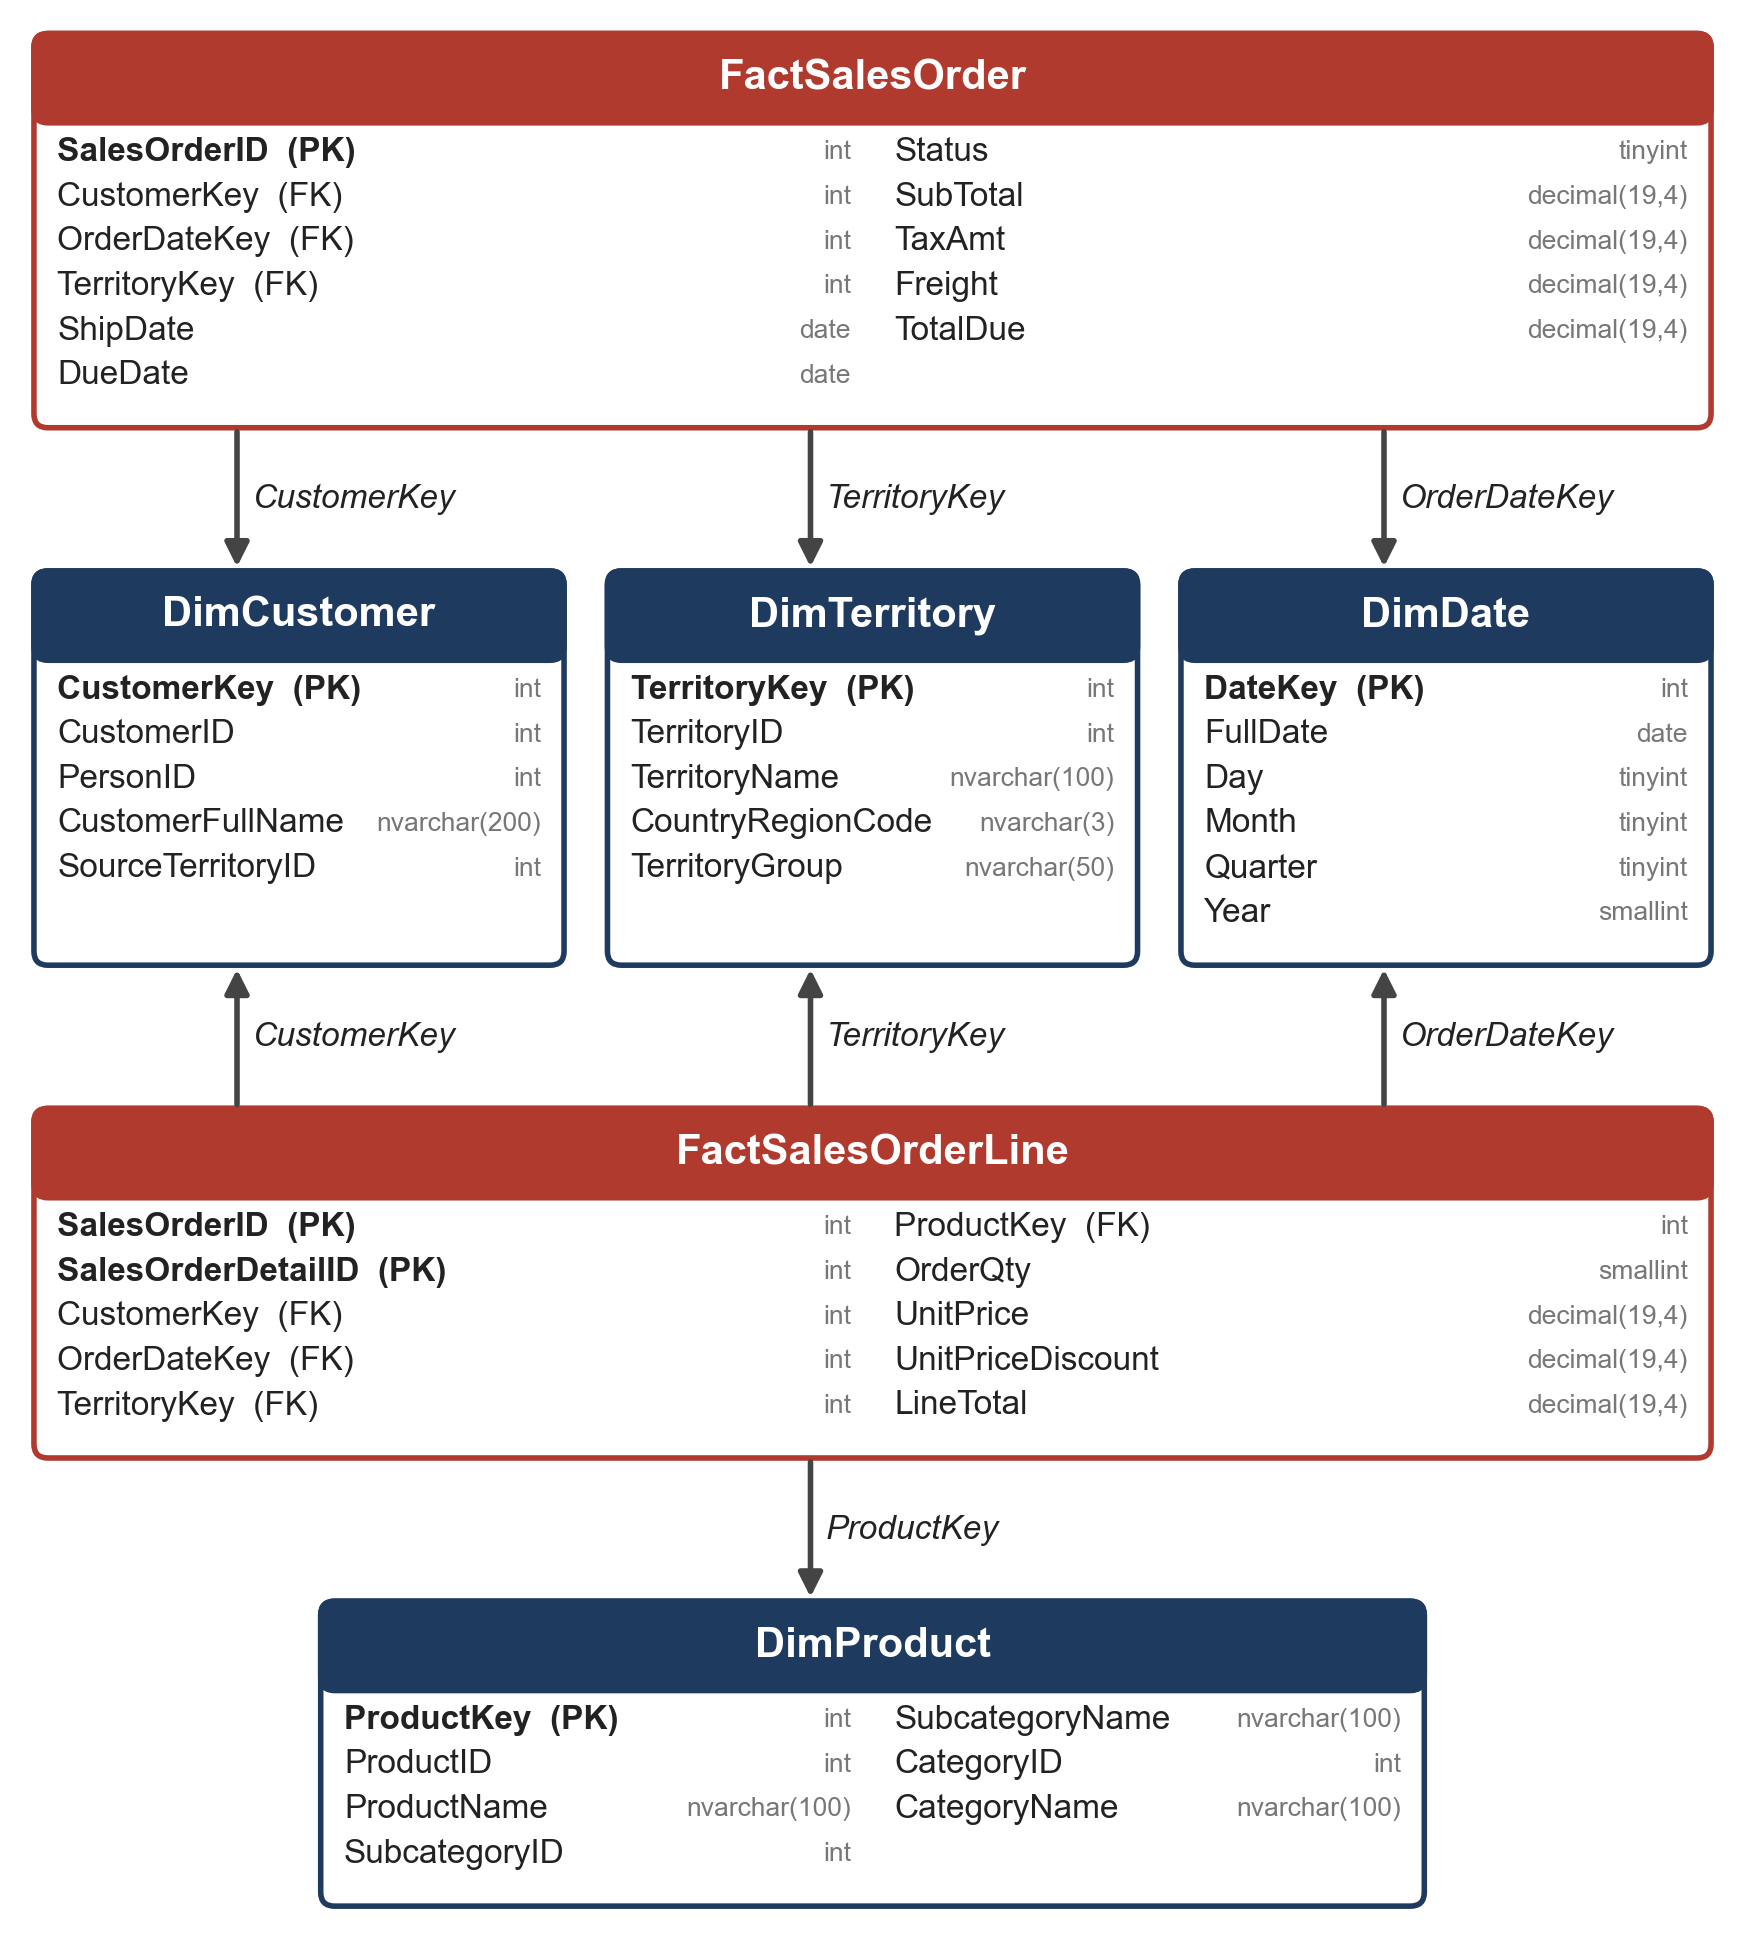
\includegraphics[width=0.5\textwidth]{luoc_do_sao.png}
\caption{Sơ đồ hình sao của kho \texttt{CompanyX\_DW}}
\label{fig:luocdosao}
\end{figure}
\subsection{Dữ liệu gốc đi vào kho như thế nào}
Bảng~\ref{tab:anhxa} cho biết dữ liệu từ bảng gốc nào đi vào bảng nào của kho và được xử lý ra sao.

\begin{table}[H]
\centering
\caption{Dữ liệu từ \texttt{CompanyX} (gốc) đi vào \texttt{CompanyX\_DW} (kho)}
\label{tab:anhxa}
\footnotesize
\begin{tabular}{p{3.8cm}p{3.0cm}p{7.6cm}}
\toprule
Bảng gốc & Bảng trong kho & Cách xử lý \\
\midrule
\texttt{Sales.Customer}, \texttt{Person.Person} & \texttt{DimCustomer} & Chỉ lấy khách cá nhân, ghép họ tên thành một cột \\
\texttt{Product}, \texttt{Product\allowbreak Subcategory}, \texttt{Product\allowbreak Category} & \texttt{DimProduct} & Ghép sản phẩm với nhóm nhỏ và nhóm lớn, vẫn giữ sản phẩm chưa phân loại \\
\texttt{Sales.SalesTerritory} & \texttt{DimTerritory} & Lấy mã vùng, quốc gia, nhóm vùng và đổi tên cột cho rõ nghĩa \\
\texttt{OrderDate} của đơn & \texttt{DimDate} & Tạo đủ mọi ngày từ ngày đặt đầu tiên đến cuối cùng, mã dạng \texttt{YYYYMMDD} \\
\texttt{Sales.\allowbreak SalesOrderHeader} & \texttt{Fact\allowbreak SalesOrder} & Chỉ lấy đơn đã gửi (\texttt{Status} bằng 5), tìm mã khách, ngày, vùng trong các bảng mô tả (vùng được để trống) \\
\texttt{Sales.\allowbreak SalesOrderDetail} & \texttt{Fact\allowbreak SalesOrderLine} & Chỉ lấy dòng của các đơn đã vào kho, tìm mã sản phẩm, giữ số lượng, đơn giá, giảm giá \\
\bottomrule
\end{tabular}
\end{table}

\subsection{Luồng ETL 11 bước}
Bảng~\ref{tab:etl11} liệt kê 11 bước của lần chạy cuối. Ở mỗi bước, số bản ghi ở cột ``Nguồn'' bằng ``Nạp'' cộng ``Loại'' cộng ``Từ chối''. Loại là bản ghi đúng nhưng không thuộc phạm vi phân tích (ví dụ khách là đại lý). Từ chối là bản ghi thuộc phạm vi nhưng bị lỗi dữ liệu.

\begin{table}[H]
\centering
\caption{Mười một bước của lần chạy ETL cuối}
\label{tab:etl11}
\footnotesize
{\setlength{\tabcolsep}{3.5pt}\begin{tabular}{rlp{4.0cm}rrrr}
\toprule
Bước & Tên bước & Việc làm & Nguồn & Nạp & Loại & Từ chối \\
\midrule
1 & \texttt{Extract.Customer} & Trích bảng khách hàng và họ tên vào staging & 19.820 & 19.820 & 0 & 0 \\
2 & \texttt{Extract.Product} & Trích sản phẩm cùng danh mục con và danh mục & 504 & 504 & 0 & 0 \\
3 & \texttt{Extract.Territory} & Trích vùng bán hàng & 10 & 10 & 0 & 0 \\
4 & \texttt{Extract.Order} & Trích đầu đơn hàng, chưa lọc & 31.465 & 31.465 & 0 & 0 \\
5 & \texttt{Extract.OrderLine} & Trích dòng chi tiết đơn, chưa lọc & 121.317 & 121.317 & 0 & 0 \\
6 & \texttt{Load.DimCustomer} & Cập nhật và bổ sung khách cá nhân & 19.820 & 18.484 & 1.336 & 0 \\
7 & \texttt{Load.DimProduct} & Cập nhật và bổ sung sản phẩm & 504 & 504 & 0 & 0 \\
8 & \texttt{Load.DimTerritory} & Cập nhật và bổ sung vùng & 10 & 10 & 0 & 0 \\
9 & \texttt{Load.DimDate} & Sinh lịch liên tục theo ngày đặt & 1.127 & 1.127 & 0 & 0 \\
10 & \texttt{Load.FactSalesOrder} & Kiểm tra rồi nạp đơn đã gửi của khách cá nhân & 31.465 & 27.382 & 4.083 & 0 \\
11 & \texttt{Load.FactSalesOrderLine} & Nạp dòng chi tiết của các đơn đã nạp & 121.317 & 59.795 & 61.522 & 0 \\
\bottomrule
\end{tabular}
}
\end{table}

\textbf{Bước 1 đến 5, lấy dữ liệu.} Sao chép nguyên bản năm bảng gốc vào vùng tạm, chưa lọc gì. Mỗi lần chạy xoá vùng tạm rồi sao chép lại.

\textbf{Kiểm tra và loại.} Trước khi lọc, nhóm kiểm tra dữ liệu ở vùng tạm: mã liên kết, ngày tháng, số tiền, số lượng, và hai phép tính tiền sau phải khớp (cho phép lệch 0,01).
\begin{align*}
\text{TotalDue} &= \text{SubTotal} + \text{TaxAmt} + \text{Freight}, \\
\text{LineTotal} &= \text{OrderQty} \times \text{UnitPrice} \times (1 - \text{UnitPriceDiscount}).
\end{align*}
Bản ghi sai được ghi vào bảng \texttt{etl.RejectedRow} kèm lý do. Nếu một dòng chi tiết sai thì cả đơn bị loại, để tổng các dòng luôn bằng tổng của đơn. Lần chạy cuối có 6 đơn và 75 dòng chi tiết sai, nhưng đều không thuộc phạm vi phân tích nên không có bản ghi nào trong phạm vi bị từ chối.

\textbf{Bước 6 đến 11, đưa vào kho.} Các bảng mô tả nạp trước, các bảng giao dịch nạp sau. Bảng mô tả chỉ cập nhật và thêm dòng nên mã số không đổi giữa các lần chạy. Phần ngoài phạm vi gồm 1.336 khách, 4.083 đơn và 61.522 dòng chi tiết. Hai bảng giao dịch được xoá hết rồi nạp lại mỗi lần chạy, vì dữ liệu của đề tài là bản sao lưu cố định. Lần chạy cuối ngày 31/10/2026 mất 2 giây và thành công (\texttt{SUCCESS}).

\subsection{Bảng Customer Snapshot}
Sau khi nạp kho, một đoạn lệnh riêng tạo bảng \texttt{analytics.\allowbreak CustomerSnapshot}, nằm ngoài sơ đồ hình sao. Mỗi dòng là tình trạng của một khách vào một ngày chốt (gọi là mốc), nhận diện bằng \texttt{CustomerID} và \texttt{SnapshotDate}. Bảng này là đầu vào của mô hình học máy. Có 19 mốc trong quá khứ (ngày 1 và 15 hằng tháng, từ 01/06/2013 đến 01/03/2014) và một mốc chấm điểm, tức ngày dùng để dự đoán cho khách hiện tại, là 08/07/2014. Tổng cộng 196.985 dòng. Chỉ số tại mốc $T$ chỉ tính từ các đơn đã đặt và đã gửi trước $T$, để mô hình không biết trước tương lai.

\subsection{Quản lý và kiểm soát chất lượng kho}
Thiết kế kho ở các mục trên cần đi kèm cách vận hành và kiểm soát kho. Các việc quản lý này đang nằm ở nhiều chương, nên mục này gom lại:
\begin{itemize}
    \item \textbf{Siêu dữ liệu và nhật ký ETL.} Bảng \texttt{etl.RunLog} ghi từng lần chạy, \texttt{etl.StepLog} ghi từng bước, \texttt{etl.RejectedRow} ghi bản ghi bị từ chối kèm lý do (Bảng~\ref{tab:etl11}).
    \item \textbf{Chiến lược làm mới.} Mỗi lần chạy nạp lại toàn bộ (full reload) bằng \texttt{etl.usp\_\allowbreak FullLoad}, trong một transaction. Nếu có lỗi, mọi thay đổi bị huỷ (rollback) như chưa từng chạy. Hạn chế của cách này nêu ở mục Giới hạn cuối chương.
    \item \textbf{Quản lý phiên bản mô hình và điểm.} Mỗi mô hình có một phiên bản trong \texttt{analytics.\allowbreak ModelRegistry}, điểm của từng khách được lưu kèm phiên bản đã chấm (mục~\ref{sec:chamdiem}).
    \item \textbf{Phân quyền theo vai trò.} Ba vai trò dùng DSS có quyền khác nhau (Bảng~\ref{tab:quyen}, mục~\ref{sec:vaitro}). Bản demo chưa có đăng nhập, vai trò chỉ chọn ở thanh bên để minh hoạ.
\end{itemize}
Về kiểm soát chất lượng, nhóm so sánh dữ liệu gốc với kho bằng câu truy vấn SQL, ở hai lớp. Lớp một gồm 44 phép kiểm tra sau khi nạp (Bảng~\ref{tab:kt44}). Ví dụ tổng tiền hàng là 29.052.549,9450 và tổng tiền đơn là 32.103.068,4755, giống nhau ở dữ liệu gốc và kho (lệch không quá 0,01). Lớp hai gồm 21 phép kiểm tra riêng cho bảng Snapshot (Bảng~\ref{tab:kt21}), tính lại chỉ số từ dữ liệu gốc rồi so với kho. Tất cả đều đạt.

\begin{table}[H]
\centering
\caption{Kết quả 44 phép kiểm tra sau khi nạp kho}
\label{tab:kt44}
\footnotesize
\begin{tabular}{lrr}
\toprule
Nhóm kiểm tra & Số phép & Kết quả \\
\midrule
Số lượng bản ghi (đầy đủ) & 8 & 8 đạt \\
Mã định danh nguồn & 8 & 8 đạt \\
Khoá và quan hệ (duy nhất, nhất quán) & 6 & 6 đạt \\
Phạm vi và ánh xạ (hợp lệ) & 8 & 8 đạt \\
Giá trị tài chính (chính xác) & 4 & 4 đạt \\
Bản ghi bất thường & 6 & 6 đạt \\
Nhật ký ETL (truy vết) & 4 & 4 đạt \\
\textbf{Tổng cộng} & \textbf{44} & \textbf{44 đạt, 0 lỗi} \\
\bottomrule
\end{tabular}

\end{table}

\begin{table}[H]
\centering
\caption{Kết quả 21 phép kiểm tra bảng Customer Snapshot}
\label{tab:kt21}
\footnotesize
\begin{tabular}{lrr}
\toprule
Nhóm kiểm tra & Số phép & Kết quả \\
\midrule
Lịch mốc & 4 & 4 đạt \\
Độ phủ khách & 4 & 4 đạt \\
Miền giá trị & 4 & 4 đạt \\
Tính lại RFM từ nguồn & 5 & 5 đạt \\
Tính lại thuộc tính sản phẩm & 4 & 4 đạt \\
\textbf{Tổng cộng} & \textbf{21} & \textbf{21 đạt, 0 lỗi} \\
\bottomrule
\end{tabular}

\end{table}

\subsection{Giới hạn}
\begin{itemize}
    \item ETL chỉ chạy khi có người bấm chạy, chưa tự chạy theo lịch, và chưa thử trường hợp lỗi giữa chừng. Một transaction cho toàn bộ ETL chỉ hợp với dữ liệu nhỏ (2 giây), dữ liệu lớn cần chia nhỏ.
    \item Chỉ có một nguồn dữ liệu, và kho ghi đè thông tin cũ nên không xem lại được thông tin trước đây.
    \item Chỉ ngày đặt hàng nối với bảng ngày.
\end{itemize}
